\documentclass[11pt]{article}
\usepackage[a4paper,margin=1.05in]{geometry}
\usepackage{amsmath,amssymb,amsthm}
\usepackage{booktabs,array,graphicx,xcolor,enumitem}
\usepackage[colorlinks=true,linkcolor=blue!50!black,urlcolor=blue!50!black,citecolor=blue!50!black]{hyperref}
\usepackage{caption}
\captionsetup{font=small,labelfont=bf}
\newcommand{\TotalCases}{6088}
\newcommand{\VerSha}{3f9bf7156c5ed7df}
\newcommand{\NPrimePairs}{195}
\newcommand{\MeanPrime}{5.6821}
\newcommand{\MaxFib}{6}
\newcommand{\NFib}{30}
\newcommand{\BfourPrime}{123993}
\newcommand{\BthreePrime}{570}
\newcommand{\BthreeA}{322}
\newcommand{\BthreeB}{721}
\newcommand{\MeanCtl}{5.3659}
\newcommand{\MeanRnd}{4.9133}
\newcommand{\NCtl}{41}
\newcommand{\NRnd}{150}

\newtheorem{theorem}{Theorem}[section]
\newtheorem{lemma}[theorem]{Lemma}
\newtheorem{proposition}[theorem]{Proposition}
\newtheorem{corollary}[theorem]{Corollary}
\theoremstyle{definition}
\newtheorem{definition}[theorem]{Definition}
\newtheorem{remark}[theorem]{Remark}
\newcommand{\N}{\mathbb{N}}
\newcommand{\dist}{\operatorname{d}}
\newcommand{\Nbr}{\operatorname{Nbr}}

\title{\textbf{Fibonacci Numbers and Primes in the Reversible\\ Square-Multiplication Graph: Structure, Distances and Selector Restrictions}\\[4pt]
\large UNNS-U2-FP \,--\, version 1.0 (v001)}
\author{UNNS Research Collective}
\date{9 November 2026}

\begin{document}
\maketitle

\begin{abstract}
\noindent Let $G$ be the graph on the positive integers in which $kN$ is joined to $k(N+1)^2$ for all $k,N\ge1$.
We prove that every prime $p$ has exactly two neighbours, $4p$ and $(p+1)^2$, so that a path between two distinct primes begins with the move $+1$ or $+p$ and ends with $-1$ or $-q$,
and that $\dist(p,q)=2+\min\dist(u,v)$ over the neighbours $u$ of $p$ and $v$ of $q$. We certify $\dist(61,67)=7$ and $\dist(661,673)=8$ by disjoint balls and explicit paths, which rules out a successor bound of $6$ for primes.
Exact distances for $\NPrimePairs$ consecutive primes below $1200$ take the values $4,\dots,8$; for $\NFib$ consecutive Fibonacci numbers they take the values $2,\dots,\MaxFib$.
Generic pairs of the same size and ratio have a comparable distribution, so these data do not by themselves exhibit special structure.
A search for two-parameter path identities along Fibonacci pairs $(F_k,F_{k+1})$ finds explicit identities, with labels that are forms in $F_k,F_{k+1}$, for the residue classes $k\equiv4,7,10\pmod{12}$ (lengths $5,7,7$); they were checked on exact pairs for every such $k<1800$, and not certified symbolically. No identity was found within the declared vocabulary for the other nine classes.
Before any construction for primes, we fix a restricted class of arithmetic selectors that separates reusable path formulas from selectors that compute the next term and then route to it. No selector for either family is constructed in this release.
\end{abstract}

\section{Introduction}\label{sec:intro}
\paragraph{Provenance.} The graph $G$ is the undirected closure of the SELECT-II transformation $m\mapsto m(N+1)^2/N$ ($N\mid m$) of the UNNS Substrate. Uniform bounds on $\dist(n,n+1)$, $\dist(n,2n)$ and $\dist(n^k,(n+1)^k)$ and finite-control selectors for the integers, the squares and fixed powers are established in~\cite{u1bnd,u2,sq}. These releases, the earlier notes~\cite{u0,u1} and the frozen reference collection~\cite{gig,repo} are unchanged.
The present release is the separate UNNS-U2-FP investigation.

\paragraph{Question.} For integers, squares and powers, two ingredients made autonomous generation possible: a uniform bound on the distance between consecutive terms, and path identities whose intermediate states determine their parameter. For Fibonacci numbers and primes, do these ingredients exist, and what must a selector be forbidden to do so that the question is not answered by simply computing the next term?

\paragraph{Results.} Section~\ref{sec:restr} fixes the selector restrictions. Section~\ref{sec:primes} proves the structure of primes in $G$ and certifies two distances. Section~\ref{sec:fib} records the Fibonacci data, the generic control and the identity search; Section~\ref{sec:pdata} the prime data; Section~\ref{sec:status} the status and the open questions.

\section{Predeclared selector restrictions}\label{sec:restr}
A \emph{selector} is as in~\cite{u2}: a finite control set $Q$ with a ready state, and a function $\Sigma(x,q)=(\pm,N,q')$ of the current integer and control state only, whose moves are legal.
An unrestricted $\Sigma$ may compute the desired next term by any algorithm; for primes that would hide the whole problem. The following class is fixed here, before any construction for primes.
\begin{definition}[Arithmetic-path selector]\label{def:aps}
A selector is an \emph{arithmetic-path selector} if
\begin{enumerate}[label=(R\arabic*),nosep]
\item $|Q|$ is finite and independent of the position in the sequence;
\item every label $N$ and every control update is given by one of finitely many \emph{label programs}: straight-line programs of bounded length over $+,-,\times$, exact division, comparison and integer roots of fixed order, applied to the current integer and to parameters recovered from it;
\item a parameter is recovered from the current integer only by inverting a strictly increasing polynomial (or an algebraic closed form fixed in advance) at the current phase, i.e.\ it is the unique preimage;
\item $\Sigma$ performs no primality test, factorization, divisor enumeration, gcd computation, search over candidate integers, or lookup of terms of the target sequence beyond a finite exceptional table;
\item the label programs are fixed by a finite list of certified path identities (each step certified by an integral positive cofactor), written down without reference to the particular terms.
\end{enumerate}
\end{definition}
The selectors of~\cite{u2,sq} are arithmetic-path selectors. The restriction is not a theorem about all selectors:
\begin{proposition}[Unrestricted comparison is empty]\label{prop:triv}
A selector with an unbounded memory register and unrestricted computation realizes every computable sequence of positive integers as raw waypoints.
\end{proposition}
\begin{proof} By connectivity of $G$~\cite{u1}, a path joins any two integers; the selector computes the next term, finds a path by breadth-first search, stores it in memory and follows it. \end{proof}
Both families must therefore be examined under Definition~\ref{def:aps}. Fibonacci numbers have an algebraic closed form for the next term, $F_{k+1}=(F_k+\sqrt{5F_k^2\pm4})/2$, which is a label program of bounded length and so is admitted by (R2). Primes have no such form, and (R4) forbids computing the next prime. Whether (R1)--(R5) can realize the primes is not claimed to be impossible; it is the open question.

\section{Primes in the graph}\label{sec:primes}
\begin{theorem}[Neighbour rigidity]\label{thm:rigid}
For every prime $p$, $\Nbr(p)=\{4p,(p+1)^2\}$.
\end{theorem}
\begin{proof} The forward moves from $p$ are $+N$ with $N\mid p$, i.e.\ $N=1,p$, giving $4p$ and $(p+1)^2$. An inverse move $-N$ needs $(N+1)^2\mid p$ with $N\ge1$, impossible as $p$ is squarefree. \end{proof}
\begin{corollary}\label{cor:ends}
A path from a prime $p$ to a prime $q\ne p$ starts with $+1$ or $+p$ and ends with $-1$ or $-q$.
\end{corollary}
(The edge $4q\to q$ is the move $-1$ with cofactor $q$; the edge $(q+1)^2\to q$ is the move $-q$.)
\begin{lemma}[Reduction]\label{lem:red}
For distinct primes $p,q$: $\dist(p,q)=2+\min_{u\in\Nbr(p),\,v\in\Nbr(q)}\dist(u,v)$.
\end{lemma}
\begin{proof} $p$ and $q$ are not adjacent, since $q\notin\{4p,(p+1)^2\}$. A shortest path is $p,u,\dots,v,q$ with $u\in\Nbr(p)$, $v\in\Nbr(q)$ and a subpath of length $\ge\dist(u,v)$; conversely $p,u,\ldots,v,q$ along a shortest $u$--$v$ path gives a walk of length $2+\dist(u,v)$. \end{proof}
Lemma~\ref{lem:red} shows that the prime problem is a problem about the four composite points $4p,(p+1)^2,4q,(q+1)^2$.

\begin{proposition}[Certified distances]\label{prop:cert}
$\dist(61,67)=7$ and $\dist(661,673)=8$.
\end{proposition}
\begin{proof} The balls $B_3(61)$ and $B_3(67)$ have $\BthreeA$ and $\BthreeB$ vertices and are disjoint, computed by two independent neighbour-enumeration programs, so $\dist(61,67)\ge7$; the path $61\to244\to1098\to12200\to5978025\to36450\to268\to67$ with moves $+1,+2,+9,+488,-162,-134,-1$ has length $7$.
The balls $B_4(661)$ ($\BfourPrime$ vertices) and $B_3(673)$ ($\BthreePrime$ vertices) are disjoint, so $\dist(661,673)\ge8$, and the path of Figure~\ref{fig:pp} has length $8$. The lower bounds are computations. \end{proof}
In particular no uniform bound $\dist(p,p^+)\le6$ holds between a prime and its successor $p^+$. This does not show that these distances are unbounded.
\begin{figure}[ht]\centering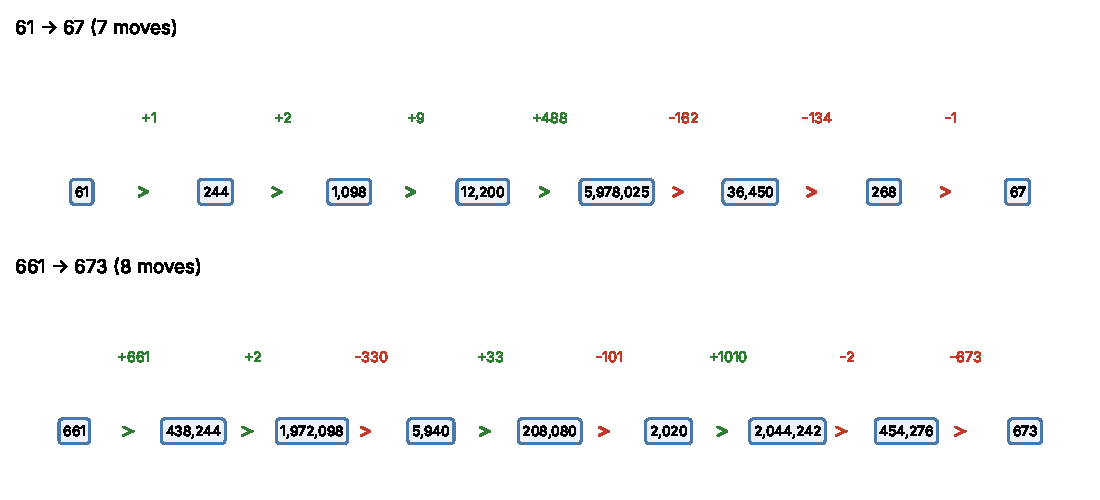
\includegraphics[width=.95\textwidth]{figures/fig3_prime_paths.pdf}\caption{Certified shortest paths between consecutive primes (green: move $+N$, red: move $-N$).}\label{fig:pp}\end{figure}

\section{Fibonacci numbers}\label{sec:fib}
\subsection{Exact data and a generic control}
Table~\ref{tab:dist} gives exact distances. A uniform bound for consecutive Fibonacci numbers was the natural target, since they satisfy a fixed recurrence; the data alone cannot support it, because pairs that are not Fibonacci but have the same size and ratio behave similarly. The rows are: the $\NFib$ resolved pairs $(F_k,F_{k+1})$, $k=2,\dots,30,32$; $\NCtl$ \emph{ratio-matched} pairs $(a,\lfloor\varphi a\rceil)$ with $a<6\cdot10^4$; the $\NPrimePairs$ consecutive prime pairs below $1200$; and $\NRnd$ random pairs below $1200$.
\begin{table}[ht]\centering\small\begin{tabular}{@{}lrrrrrrrr@{}}\toprule family & pairs & $d{=}2$ & 3 & 4 & 5 & 6 & 7 & 8\\\midrule
consecutive Fibonacci & 30 & 1 & 0 & 3 & 17 & 9 & 0 & 0 \\
ratio-matched generic pairs & 41 & 0 & 0 & 4 & 18 & 19 & 0 & 0 \\
consecutive primes $<1200$ & 195 & 0 & 0 & 8 & 62 & 110 & 14 & 1 \\
random pairs $<1200$ & 150 & 0 & 4 & 37 & 81 & 24 & 4 & 0 \\
\bottomrule\end{tabular}
\caption{Exact distances (histograms). The pairs $F_{31},F_{33},F_{34},F_{35}$ exceeded the time limit and are not included; neither are four ratio-matched pairs that exceeded a 25-second limit.}\label{tab:dist}\end{table}
\begin{figure}[ht]\centering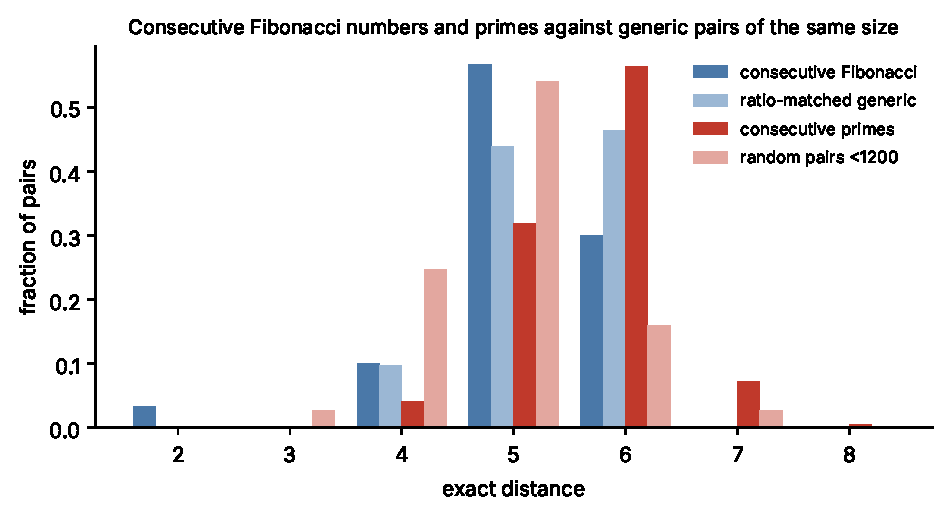
\includegraphics[width=.8\textwidth]{figures/fig1_distributions.pdf}\caption{Normalized distance distributions.}\end{figure}
Means: ratio-matched pairs $\MeanCtl$, random pairs $\MeanRnd$, consecutive primes $\MeanPrime$.

\subsection{A search for two-parameter identities}\label{sec:fibsearch}
For the successor, squares and powers, the path identities had labels polynomial in one parameter. For Fibonacci pairs $x=F_k$, $y=F_{k+1}$ the natural analogue is a path from $x$ to $y$ whose labels are forms in $x,y$ and that is valid for all $k$ in a residue class (the Pisano period of $24$ is $24$).
We searched by meeting in the middle over state tuples at three test pairs per class, with a vocabulary of about $300$ forms $(ax+by+c)/d$ and a few small products, up to seven moves. The same tool recovers the known successor identity of class $24t+19$ (record in \texttt{reports/search\_sanity.json}).
\begin{proposition}[Found families, computationally supported]\label{prop:fibfam}
For $k\equiv4\pmod{12}$ the moves
\[ +1,\ +x,\ +\tfrac{x+3y-2}{4},\ -(2y-x+2),\ -y \]
carry $x=F_k$ to $y=F_{k+1}$ legally in five moves. For $k\equiv7$ the seven moves $+x,\ +(2x+y+2),\ -\tfrac{3x-y-2}{4},\ -\tfrac{y-3}{2},\ -1,\ +\tfrac{y-3}{6},\ -\tfrac y3$ and for $k\equiv10$ the seven moves
$+1,\ +4,\ +x,\ +\tfrac{x+3y-2}{4},\ -(2y-x+2),\ -4,\ -y$ do the same. Every label is a positive integer and every move is legal for every such $k<1800$ (check F8).
\end{proposition}
This is a statement about $150$ values of $k$ in each class, with numbers up to about $10^{375}$; it is \emph{not} proved for all $k$. A proof would need divisibility on the variety $y^2-xy-x^2=(-1)^k$ rather than polynomial division. The case $k\equiv4\pmod{12}$ has a recognizable origin: the last label $2y-x+2=L_k+2$ equals $L_{k/2}^2$ for $k\equiv0\pmod4$ (Lucas numbers $L_j$), checked for these $k$.
Thus a uniform bound is suggested for one quarter of the indices, with length $5$ on one class and $7$ on two; for the other nine classes mod $12$ the search found no identity in its vocabulary, which says nothing about whether one exists: richer labels (e.g.\ $F_{2k}=F_kL_k$, $F_{2k+1}=F_k^2+F_{k+1}^2$) were not in the vocabulary.

\section{Primes: data and structure}\label{sec:pdata}
Exact distances for consecutive primes below $1200$: see Table~\ref{tab:dist}. The pairs at distance $\ge7$ are \begin{center}$(61,67)$, $(157,163)$, $(271,277)$, $(397,401)$, $(457,461)$, $(541,547)$, $(607,613)$, $(661,673)$, $(751,757)$, $(757,761)$, $(991,997)$, $(997,1009)$, $(1051,1061)$, $(1117,1123)$, $(1171,1181)$.\end{center}
\begin{figure}[ht]\centering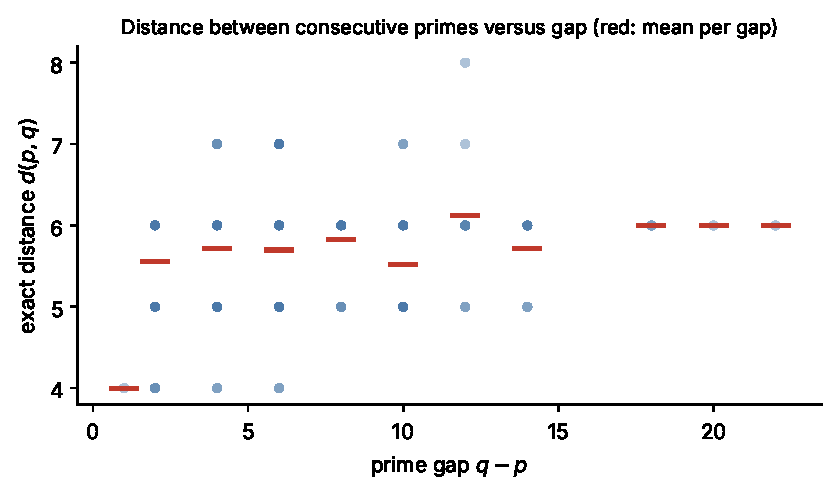
\includegraphics[width=.72\textwidth]{figures/fig2_gap.pdf}\caption{Exact distance against the gap between consecutive primes.}\end{figure}
The distance tends to be larger for larger gaps, but the range is small and the data are not a theorem. Together with Theorem~\ref{thm:rigid}, a prime selector must at each prime waypoint choose between exactly two moves, $+1$ or $+p$, and its arrival move is one of two; no prime-search algorithm is needed to state this restriction, and none is used here.

\section{Status and open questions}\label{sec:status}
\begin{table}[ht]\centering\small
\begin{tabular}{@{}p{0.36\textwidth}p{0.17\textwidth}p{0.37\textwidth}@{}}\toprule
statement & status & basis\\\midrule
neighbour rigidity, reduction lemma & proved; checked & Thm.~\ref{thm:rigid}, Lem.~\ref{lem:red}; F1, F2\\
$\dist(61,67)=7$, $\dist(661,673)=8$ & computation & disjoint balls, two engines, explicit paths; F3\\
prime and Fibonacci tables & computation & F4, F5 (second engine on a prefix)\\
generic control & record & F6\\
Fibonacci identities, $k\equiv4,7,10\pmod{12}$ & computation, uncertified & validated for $k<1800$; F7, F8\\
other nine classes & none found in the vocabulary & F7\\
selector for Fibonacci numbers & not constructed & --\\
selector for primes & not constructed & --\\
formal certification, originality review & not done & --\\\bottomrule
\end{tabular}
\caption{Status. All verifier checks passed (\TotalCases{} cases; verifier hash prefix \texttt{\VerSha}).}\end{table}
\paragraph{Open questions.}
\begin{enumerate}[nosep]
\item Is $\dist(F_k,F_{k+1})$ bounded for all $k$? Can the three found families be proved for all $k$, e.g.\ by ideal membership on $y^2-xy-x^2=\pm1$? Do identities with richer labels (Lucas numbers, index-doubling formulas, divisibility $F_k\mid F_{jk}$) cover the other nine classes, and can the parameter be recovered from the current state under (R3)? For the families found, the intermediate states are polynomials in $x,y$, and their monotonicity in $k$ has not been examined.
\item Is $\dist(p,p^+)$ unbounded? Is there any arithmetic-path selector (Definition~\ref{def:aps}) for the primes, or does (R4) together with Theorem~\ref{thm:rigid} exclude one?
\item Does a generic pair of comparable size have uniformly bounded distance, so that boundedness for Fibonacci numbers or primes would carry no information?
\end{enumerate}

\appendix\section{Reproducibility}
From \texttt{code/}: \texttt{python3 verify\_u2\_fp.py --out ../reports/u2\_fp\_verification\_report.json --data ../data} (about fifteen minutes; run without \texttt{-I}). \texttt{u1\_bnd\_lib.py} is an unchanged copy from the earlier releases; \texttt{mitm.py} extracts paths by meeting in the middle; \texttt{fibparam.py} is the identity search; \texttt{fib\_table.py} and \texttt{primescan.py} generate tables with time limits. The earlier verifications are not re-run (see the README).

\begin{thebibliography}{9}
\bibitem{u0} UNNS Research Collective, \emph{UNNS-U0: Arithmetic reachability and orbit admissibility}, research note U0-001, 8 November 2026 (local release; not part of the frozen repository).
\bibitem{u1} UNNS Research Collective, \emph{UNNS-U1: Reversible arithmetic connectivity}, research note, 8 November 2026 (provisional baseline; local release).
\bibitem{u1bnd} UNNS Research Collective, \emph{Bounded Successor Distance in the Reversible Square-Multiplication Graph}, UNNS-U1-BND version 1.0 (v001), 8 November 2026 (local release).
\bibitem{u2} UNNS Research Collective, \emph{Intrinsic Generative Selectors: Finite Control, Arithmetic State, and Observational Realization}, UNNS-U2-001 version 1.0 (v001), 8 November 2026 (local release).
\bibitem{sq} UNNS Research Collective, \emph{Squares and Power Sequences in the Reversible Square-Multiplication Graph}, UNNS-U2-SQ version 1.0 (v001), 9 November 2026 (local release).
\bibitem{gig} UNNS Research Collective, \emph{UNNS Generative Information Geometry collection}, frozen release, repository \texttt{ukbbi/UNNS}, commit \texttt{a115e4bc6b8ee734e6146b3b17a6b121e65d31c3}:
\url{https://github.com/ukbbi/UNNS/tree/a115e4bc6b8ee734e6146b3b17a6b121e65d31c3/projects/UNNS_Generative_Information_Geometry}.
\bibitem{repo} UNNS project repository, pinned at the same commit:
\url{https://github.com/ukbbi/UNNS/tree/a115e4bc6b8ee734e6146b3b17a6b121e65d31c3}.
\end{thebibliography}
\end{document}
